
To enhance the sensitivity to the Higgs boson signal, we apply additional 
$m_{\rm{H}}$ hypothesis dependent selections on the the following three variables:

%%%%%%%%%%%%%%%%%%%
\begin{enumerate}
\item $\met$ 
\item Higgs transverse mass ($M_{T}$ in Eq.~\ref{eq:MTHZZ})
\item $\Delta\phi$ between the $\met$ and the nearest jet if the jet $\Et > 30\ \GeV$, referred to as $\Delta\phi(jet,met)$.
\end{enumerate}
%%%%%%%%%%%%%%%%%%%

The selection on the $\Delta\phi(jet, met)$ is introduced to reduce the \dyll\ background, where the 
\met\, is mainly due to the jet mis-measurement. The optimization of the selections on the 
above 3 variables are described in Ref.~\cite{HZZ2011EPS}, with the lateset 
values shown in Ref.~\cite{hzzcutbase}. 
%Tables \ref{tab:HiggsSelectionCutBased} shows the expected 

%%%%%%%%%%%%%%%
\begin{figure}[!hbtp]
\begin{center}
\label{fig:mtemloosesel}
\subfigure[0-Jet]{\label{subfig:dphijetmet}
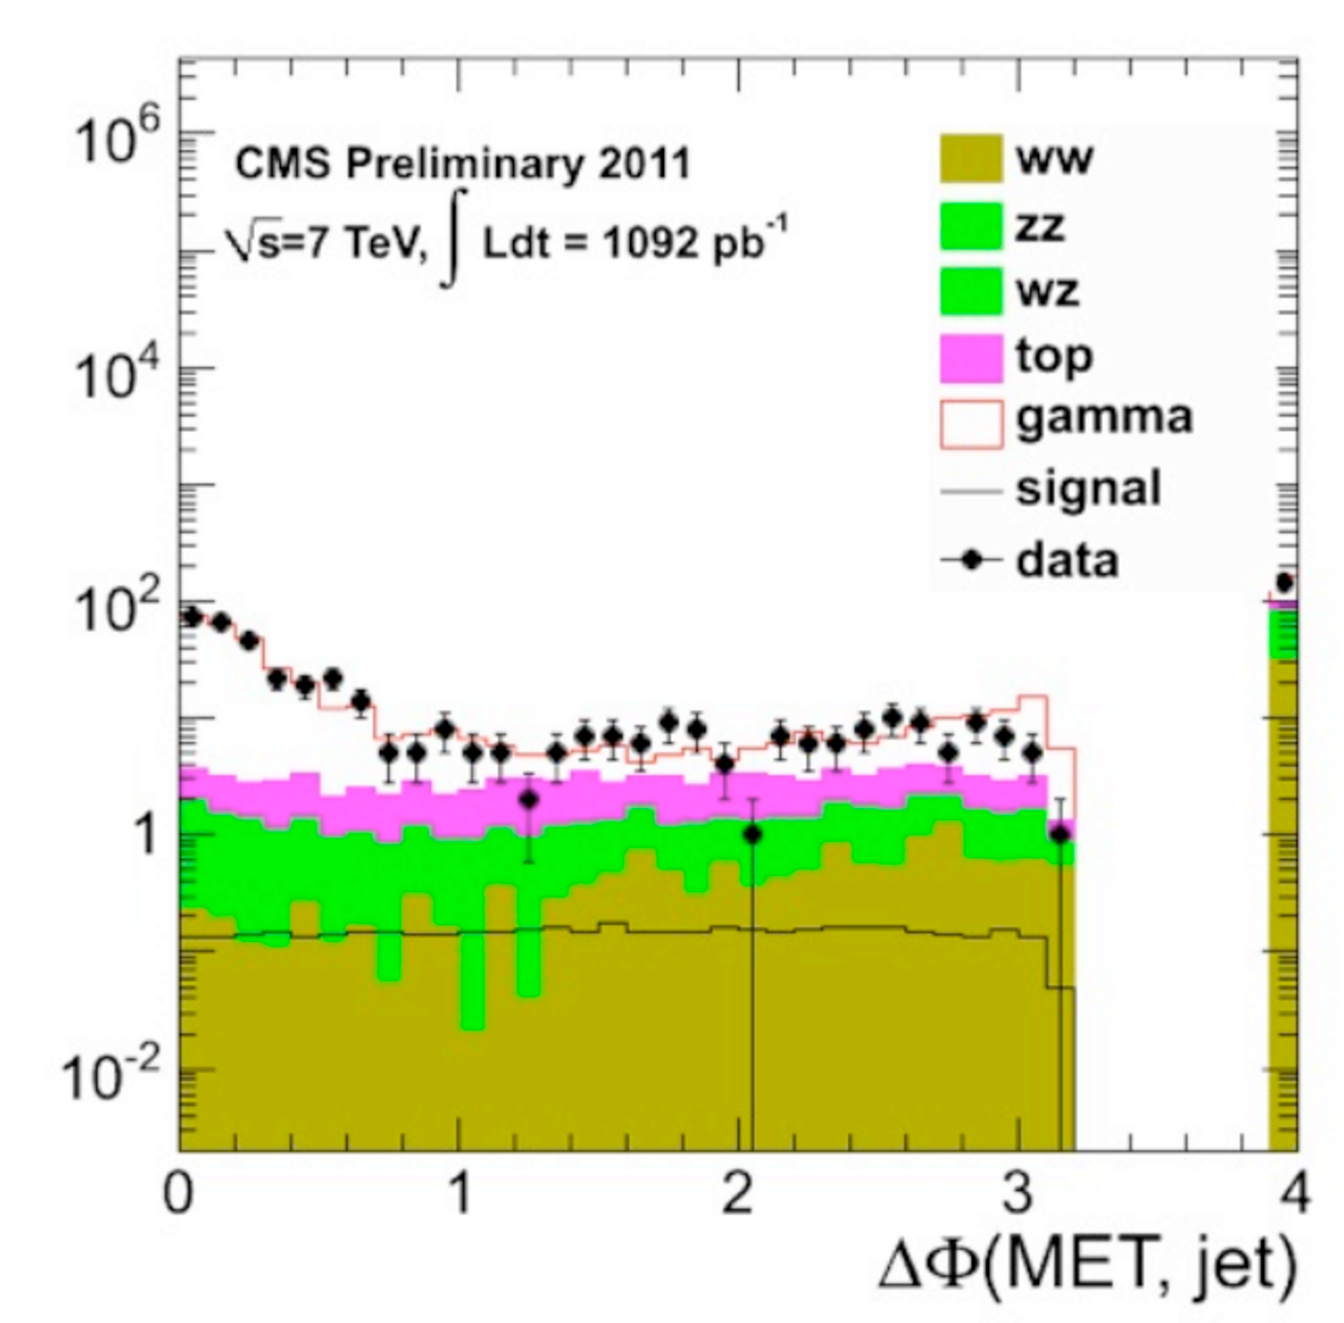
\includegraphics[width=0.5\textwidth]{figures/dphijetmet.pdf}}
\caption{The $\Delta\phi(jet,met)$ between the \met\, and the nearest jet ( with $\Et>30\,\GeV$). }
\end{center}
\end{figure}
%%%%%%%%%%%%%%%



%The higgs selection cuts are optimized for the significance ($S/\sqrt{S+B}$)
%separately in the 0-jet and 1-jet. The values of the cuts are summarized in
%Tables \ref{tab:HiggsSelectionCutBased_0j} and \ref{tab:HiggsSelectionCutBased_1j} for the 0-jet and 1-jet bins. 
%A one sided cut is applied on the minimum \met and a two sided cut is applied on the transverse mass. 

%%%%%%%%%%%%%
%\begin{table}[!ht]
%\begin{center}
%\begin{tabular}{c|c|c|c}
%\hline
%Higgs Mass        & Min $\met$ Cut Value  & Min $\mt$ Cut Value   & Max $\mt$ Cut Value \\ 
%\hline 
%250               & $> 60$ GeV            & $> 220$ GeV            & $< 260$ GeV          \\ \hline 
%300               & $> 70$ GeV            & $> 260$ GeV            & $< 320$ GeV          \\ \hline 
%400               & $> 70$ GeV            & $> 260$ GeV            & $< 320$ GeV          \\ \hline 
%\end{tabular}
%\caption{Higgs selections in the cut-based analysis.}
%\label{tab:HiggsSelectionCutBased_0j}
%\end{center}
%\end{table}
%%%%%%%%%%%%%

%Due to the missing VBF production samples for the signal in our Spring11 set of 
%Monte Carlo samples,  we did not include the yields for the VBF contribution. 
%In Table \ref{tab:VBFSignalContribution} we summarize the expected VBF contribution to the signal yield
%estimated from the Summer11 Monte Carlo samples.
%We do not perform any scaling based on these expectations.
%Because we could not make a meaningful choice of cuts for the 2-jet bin,
%we temporarily dropped it from this analysis.

%%%%%%%%%%%%%%
%\begin{table}[!ht]
%\begin{center}
%\begin{tabular}{|c|c|c|}
%\hline
%Higgs Mass        & Relative VBF Contribution in 0-Jet Bin & Relative VBF Contribution in 1-Jet Bin \\ 
%\hline 
%250               & $1.8\%$                                & $11\%$                                 \\ 
%300               & $1.9\%$                                & $9.8\%$                                \\ 
%\hline 
%\end{tabular}
%\caption{Expected relative contribution from the VBF production process to the total
%expected signal yield.}
%\label{tab:VBFSignalContribution}
%\end{center}
%\end{table}
%%%%%%%%%%%%%


%% The quoted results in this section are scaled to 1 $\ifb$ of integrated luminosity. 
%% The background yields have been scaled taking into account the observed data 
%% corrections, discussed in Section~\ref{sec:backgrounds}, with the current data 
%% sample to give realistic estimations, while $gg \to H \to ZZ$ simulated 
%% events are reweighted to match the Higgs $\pt$ at NNLO, as explained in 
%% Section~\ref{sec:datasets}. 

%% Stuff to add in the MVA later
%To enhance the sensitivity to the Higgs boson signal, two different approaches 
%are performed. The first one is a cut-based approach where further requirements 
%on a few observables are applied, while the second one makes use of
%multivariate techniques. Both of them cover a large Higgs boson mass
%($m_{\rm{H}}$) range, and each is separately optimized for different
%$m_{\rm{H}}$ hypotheses. The first method is the simplest approach with smaller
%systematic uncertainties. The second one is
%more powerful, since it exploits the information present in the
%correlation among the variables. 

%Output of the multivariate discriminator has two different use
%cases. In the first case we use it as just one more variable to cut on
%in the cut-based analysis. In the second case we use the discriminator
%output distribution for the final signal extraction.

%All analyses are further split in the corresponding 0-jet, 1-jet and
%2-jet bins. In the 2-jet bin we use a simple cut-based approach for
%now due to the limited sensitivity and the limited number of events in
%simulation.

